%
%
% begin of preamble
\input{00_preamble/preamble}
% end of preamble
% 
% begin of document

\begin{document}
\begin{flushright}
\includegraphics[width=3cm]{Logos/logo_epfl_coul-crop}
\end{flushright}

\vspace{1cm}

\begin{center}

\vspace{1cm}

\LARGE
\# Travel: Shared topics among locations

\vspace{2cm}

Automatically detect topics in the city and the associated
locations

\vspace{1cm}

%\begin{figure}[H]
%\centering
%\includegraphics[width=0.6\textwidth]{Images/skyplot}
%\caption{HERE_TEXT}
%\label{fig:skyplot}
%\end{figure}
\large

\vspace{0.5cm}

Optional Semesterproject by Renato Kempter\\

\vspace{0.5cm}

Supervised by Dr. Pearl Pu

Laboratory of Human Computer Interaction

\vspace{1cm}

08.01.2015\\


\end{center}
\normalsize
\newpage
\tableofcontents
\newpage
\section{Abstract}
We often have a subject, a taste, a style or an interest that guides us to locations we like.  Using geo-localized photos from instagram and their associated hash-tags, we propose a batch processing system that: a) Automatically clusters a set of instagrams based on the geographical coordinates, b) Extracts the most trending topics and c) Finally generates sets of locations that share the same topic. Through a web application, users can then browse the different topics and their corresponding locations.

\section{Introduction}
Instagram\footnote{\url{http://www.instagram.com}} is a mobile application used to upload photos and share them with friends and followers. Users have the ability to attach hash-tags to the posted image, that have a categorical function and cluster similarly tagged photos together. Optionally, photos can be geo-localized, either using a location name or coordinates from the integrated GPS of the device. Instagram is a highly popular mobile application with over $300$ million users. Instagrams can be published either privately or to the entire world. For the second choice, there exists an API (Application Programming Interface) that allows access to all publicly posted instagrams\footnote{\url{http://instagram.com/developer/}}.

Due to its large user base, instagrams are published all over the world and the application is heavily used while traveling\footnote{\url{https://www.yahoo.com/travel/forget-selfies-instagram-actually-makes-traveling-99392573317.html}}. Because of the quantity of data accessible through the API and the recent success of startups (e.g. JetPac\footnote{\url{http://www.jetpac.com/}}, acquired by Google) using the user generated content to aggregate additional information about locations, we were motivated to extract sets of location that share a common topic. A topic is similar to a description using a bag of words. An example for a topic we extracted from our data set is "design, vintage, deco". Using topics for travel recommendation has multiple advantages:
\begin{enumerate}
  \item Topics can be dynamic: Compared to both tags and categories, which characterize a location, topics can change over time and are an aggregation of locations. From our data set, we were able to extract topics such as "Christmas" or "snow", "cold" and "fall".
  \item A list of locations having something in common is an approach that has been used widely in different other areas, such as in music (Spotify Playlists) or fashion\footnote{\url{http://www.polyvore.com}}. In the area of traveling, different startups and established companies are trying to motivate people to create such lists (e.g. Airbnb\footnote{\url{http://www.airbnb}}).
\end{enumerate}

Users publishing a photo with a location attached often add hash-tags to describe the taken picture, the location or the mood. Our work is based on the assumption that the location where the picture was taken and the description with hash-tags are related. In other terms, we assume that the used hash-tags are a description of the location. We are well aware that this might not always be the case (for example, in the case where access is only possible through wifi and people tag all their photos with the place where they are while posting instead of where they took it). We try to consider this by preprocessing the data set carefully. The report is structured in the following way. First, we present related work, characterize our extracted dataset, present the algorithm and architecture, followed by results and the conclusion.

\section{Related work}
For the domain of travel planning, not many related papers have been published so far. J-F. Bérubé et al. \cite{berube2006time} solves the travel planning problem by computing time-dependent shortest paths through a fixed sequence of nodes. Their work focuses mainly on optimizing the visit of a given set of nodes in order to see more. Their work divers from ours in the sense that our recommendations are based on topics. Yu Zheng et al. \cite{yuzhen} propose the mining of GPS traces in order to generate two types of travel recommendations. The first type is a generic one, that recommends interesting travel locations and sequences in a given geospatial area. The second type are personalized recommendations matching the travel type. They introduce tree-based hierarchical graphs to model users' location histories and propose a Hypertext Induced Topic Search based model to infer the interest level of a location. For personalized recommendations, collaborative filtering methods are used. The used dataset differs significantly from ours. Compared to GPS traces, traces of instagrams suffer from sparsity. Shuangyu Yu et al. \cite{Yu:2014:PDJ:2678534.2678823} use a Instagram as their data source to recommend Hot Travel Routes. They present a novel concept, called Journey Group (JG), which is a group trajectory pattern reflecting a large number of users who walk through a common trajectory and present a novel Journey Group Trajectory Patterns mining strategy from user generated content based data. Part of their architecture and data cleaning is similar to ours. The processing of clusters differs from ours in the sense that they generated trajectory information based on timestamps and users with multiple instagrams. Our data analysis showed that such an approach can induce a bias. We therefore worked with textual content of instagrams instead.


\section{Data Format}
\label{sct:data}

The dataset of instagrams has a total size of over $712485$ geo-located instagrams out of the environment from Paris, including Saint-Denis, Colombes and Versailles. The data has been captured between the $12$th of October 2014 until the $10$th of December 2014. The majority of the data is coming from the center of Paris. A subset of the data and its distribution using Google Fusion Tables and Google maps can be found here\footnote{\url{http://bit.ly/1tKjrcX}}. The vast majority of clusters is located in the center of Paris.

The data is retrieved in real-time from the Instagram servers. The Instagram API \footnote{\url{http://instagram.com/developer/realtime/}} has adapted parts of the Pubsubhubbub protocol \footnote{\url{https://en.wikipedia.org/wiki/PubSubHubbub}}, which allows being notified when a new photo was posted in a certain geographical area. Currently, our application does not take advantage of the real-time capabilities, as it requires changes in the infrastructure.

Each instagram has the following attributes:
\begin{enumerate}
  \item Id - A unique value that identifies the instagram
  \item user\_name - the author name of the instagram
  \item user\_id - the id of the user
  \item tags - A set of tags attached by the user to describe the taken photo
  \item location\_name - users can attach a location name indicating the place where the photo was taken
  \item location\_lat - geographical latitude where the photo was taken
  \item location\_lng - geographical longitude where the photo was taken
  \item filter - chosen filter for the photo
  \item created\_time - Date \& Time when the photo was posted
  \item image\_url - Url to the image
  \item media\_url - Url to the instagram (including likes, text and comments)
  \item text - The text attached to the instagram
\end{enumerate}

While all the photos have geographical coordinates (latitude and longitude), only a third of the data contains data for the location\_name. We tried to correlated the location\_name column to the foursquare database and identified $10826$ different venues in Paris that were mentioned in instagrams. For all those venues, we retrieved through the application programming interface (API) of Foursquare additional information, including: the exact coordinates, the address, category, the price level (between 1 and 4) as well as different statistics, such as rating, count of check-ins, likes and tips.

\subsection{Exploratory Data analysis}

In this section, we describe the basic characteristics of the dataset. Only a subset ($84531$ instagrams) of the large dataset has been augmented with foursquare data.

\subsubsection{Location information}

Users can add the location name to their posting. This is quite a popular feature ($302164$ instagrams have a location\_name out of $712485$), making up $42.4\%$ percent of the data. Users can either select a place out of a list of locations or create the place themselves. Unfortunately, this introduces some noise and leads to ambiguities, because popular locations exist in different names for different languages. Furthermore, some users abuse the feature to post SPAM and advertisement messages. As stated in section \ref{sct:data}, we decided to pre-process and normalize the column location\_name by correlating the received location names with another popular venue service called Foursquare\footnote{https://foursquare.com/}. Foursquare has as instagram an API, that allows search for venues given a query and coordinates.

\paragraph{Most mentioned location names}

The distribution of location names follows a Zipfian distribution, as one can clearly see in the log-log plot in figure \ref{fig:location_name_log_log}. The locations are listed in Table \ref{table:top_places}.

\begin{figure}[h!]
  \centering
    \includegraphics[width=0.5\textwidth]{images/location_name_distribution_log_log}
  \caption{Log-Log plot of rank and frequency of hashtags}
  \label{fig:location_name_log_log}
\end{figure}

\begin{table}
  \centering
  \begin{tabu}{| l | l |}
  \hline
  Tour Eiffel & 12379 \\ \hline
  Paris, France & 9856 \\ \hline
  Musée du Louvre & 9028 \\ \hline
  Fondation Louis Vuitton & 4474 \\ \hline
  Cathédrale Notre-Dame de Paris & 3713 \\ \hline
  Centre Pompidou & 3664 \\ \hline
  Paris & 2607 \\ \hline
  Château de Versailles & 2533 \\ \hline
  Sacré-Coeur, Paris & 2507 \\ \hline
  Galeries Lafayette & 2144 \\ \hline
  Tour Eiffel - Place Du Trocadero & 1982 \\ \hline
  Eiffel Tower & 1826 \\ \hline
  Jardin des Tuileries & 1794 \\ \hline
  Paris Bercy (Officiel) & 1748 \\ \hline
  Place de la concorde & 1671 \\ \hline
  Montmartre & 1628 \\ \hline
  Jardin du Luxembourg & 1610 \\ \hline
  Champs Elysees Paris & 1449 \\ \hline
  Grand Palais Paris & 1232 \\ \hline
  Avenue des Champs-Elysées & 1206 \\ \hline
  \end{tabu}
  \caption{Top $20$ most mentioned places}
  \label{table:top_places}
\end{table}

\paragraph{Venues} The locations that are left over after having pre processed the location\_name column are the venues. For all venues, we have additional data, such as the category and price level, exact coordinates and statistics about check-ins. Mostly, we were interested in knowing the distribution of categories of venues, as showed in figure \ref{fig:category_distribution}. The amount of streets, homes, office and hotels is surprisingly high.

\begin{figure}[h!]
  \centering
    \includegraphics[width=0.5\textwidth]{images/category_distribution}
  \caption{Distribution of categories of locations}
  \label{fig:category_distribution}
\end{figure}

\subsubsection{User information}

In this section, we'll describe the characteristics of users in the dataset. The dataset has a total of $162'972$ users. Each user takes on average $4.4$ instagrams. The median is $2$, standard deviation is $9.35$. Minimum is equal to $1$, maximum equal to $937$. The first $10'000$ users can be modeled by a power law distribution, as it is observable in figure \ref{fig:user_instagram}. The low median explains the strong drop after user of rank $10^4$. $50\%$ of the users have taken 2 or less instagrams during their trip. 

\begin{figure}[h!]
  \centering
    \includegraphics[width=0.5\textwidth]{images/user_instagram_log_log}
  \caption{Distribution of instagram's per user}
  \label{fig:user_instagram}
\end{figure}

\subsubsection{Graph analysis}

Based on the correlated location data and the fact that some users have taken multiple photos, we generated an undirected graph. A node is equal to a venue, whereas an edge means that a person has taken an instagram at both places. The weight of an edge is equal to the number of people that have posted an instagram at both locations. As we are using the venue data, only a sample of about $84531$ of the original data is used. Interestingly, after building the graph, we find $233$ different disconnected components. The main component has $6414$ nodes, while the other $232$ subgraphs have a maximum of $4$ nodes (most of them have only $2$ nodes). For the following investigations, we discarded all disconnected components and kept only the main one.

\paragraph{Edge distribution and weights}
There is a total of $54033$ edges in the graph. Mean of edge weight is equal to $27.18$, median $2$, standard deviation $469.77$, minimum $1$ and maximum $19272$. In figure, one can see the distribution of edge weights. The connected nodes of the top edges are listed in table \ref{table:edges}. 

\begin{table}
  \centering
  \begin{tabularx}{\textwidth}{| X | X | X |}
    \hline
    \textbf{Edge weight} & \textbf{Node 1} & \textbf{Node 2} \\ \hline
    729 & Musée du Louvre & Pont Alexandre III | Paris, FRA \\ \hline
    502 & Tour Eiffel & Le Jules Verne \\ \hline
    297 & Métro Porte de Versailles [12] & Place de la Porte de Versailles \\ \hline
    246 & Parvis de Notre-Dame & Musée du Louvre \\ \hline
    207 & Place du Trocadéro & Tour Eiffel \\ \hline
    201 & Tour Eiffel & Château de Versailles \\ \hline
    190 & Bibliothèque des Arts Décoratifs & Les Arts Décoratifs \\ \hline
    171 & Tour Eiffel & Musée du Louvre \\ \hline
    156 & paris drobs flat & Les Citadines \\ \hline
    149 & Salon du Chocolat de Paris & Métro Porte de Versailles [12] \\ \hline
    145 & Park \& Suites Grande Bibliotheque Hotel Paris & Musée du Louvre \\ \hline
    140 & C.C Saint-Lazare Paris & Café Marco Polo \\ \hline
    131 & Jardin d'Acclimatation & Fondation Louis Vuitton \\ \hline
    128 & Le Florence & 101 Taipei \\ \hline
    110 & Café Pasteur & Institut Pasteur \\ \hline
    108 & Musée du Louvre & Musée National Gustave-Moreau \\ \hline
    108 & La Paillasse & Carreau du Temple \\ \hline
    106 & Musée du Louvre & Pont des Arts \\ \hline
    104 & Arrêt Cité Palais de Justice & Musée National Gustave-Moreau \\ \hline
    99 & Salon du Chocolat de Paris & Place de la Porte de Versailles \\ \hline
    \hline
  \end{tabularx}
  \caption{Top edges in terms of weights and their associated nodes}
  \label{table:edges}
\end{table}

\paragraph{Edge length}
We were interested in knowing about the length of the edges, meaning the distance in meters between two instagrams taken by a users. We plotted two different figures: In figure \ref{fig:unweighted_edge_distance}, every edge is only counted once, while in figure \ref{fig:weighted_edge_distance}, each edge is counted its weight times. From comparison of the two figures, short edges have proportionally higher weights than longer edges. We have the following characteristics: Mean = $3433.18$m, Median = $2586.77$m, maximum distance = $22153.2$m, minimum distance = $0$m. The maximum distance is from the center of Paris to Versailles.

\begin{figure}[h!]
  \centering
    \includegraphics[width=0.5\textwidth]{images/unweighted_edge_distance}
  \caption{Histogram of edge length. Every edge is counted only once.}
  \label{fig:unweighted_edge_distance}
\end{figure}

\begin{figure}[h!]
  \centering
    \includegraphics[width=0.5\textwidth]{images/weighted_edge_distance}
  \caption{Histogram of edge length. Every edge is counted $weight$ - times}
  \label{fig:weighted_edge_distance}
\end{figure}

\paragraph{Degrees of nodes}
The degree of a node is the number of edges incident to the node \footnote{\url{https://en.wikipedia.org/wiki/Degree_\%28graph_theory\%29}}. In our graph, the degree of a node is equal to the number of Instagrams taken at a location (multiple instagrams by a user at a location count as one). In figure \ref{}, once can see that the most popular touristic places in Paris have also the highest degree in the graph.

\begin{table}
  \centering
  \begin{tabu}{| l | l |}
    \hline
    \textbf{Location} & \textbf{Degree} \\ \hline
    paris & 148190 \\ \hline
    love & 33049 \\ \hline
    france & 32439 \\ \hline
    instagood & 18081 \\ \hline
    picoftheday & 16081 \\ \hline
    fashion & 15723 \\ \hline
    photooftheday & 15293 \\ \hline
    beautiful & 12822 \\ \hline
    art & 11216 \\ \hline
    friends & 11017 \\ \hline
    tagsforlikes & 10831 \\ \hline
    girl & 10678 \\ \hline
    vscocam & 10667 \\ \hline
    food & 10487 \\ \hline
    happy & 10469 \\ \hline
    followme & 10105 \\ \hline
    instadaily & 9843 \\ \hline
    igers & 9723 \\ \hline
    me & 9601 \\ \hline
    follow & 9373 \\ \hline
    \hline  
  \end{tabu}
  \caption{The 20 most popular hash-tags in the dataset}
  \label{tbl:hashtags}
\end{table}

\subsubsection{Communities}

We also looked at the structure of communities inside the graph. For this, we used the Louvin Community detection algorithm proposed by V. Blondel and al. \cite{blondel2008fast}. It is implemented for the Python Networkx Package\footnote{{https://networkx.github.io/}} \footnote{\url{https://bitbucket.org/taynaud/python-louvain}}, as well as for Gephi\footnote{https://gephi.github.io/}. The outcome was highly interesting: Most of the detected communities were extremely small ($4-5$ locations only), but there were 3 communities that had $321$, $398$ and $538$ locations. After further analysis of the geographical and categorical structure of those big communities, we were not able to find a specific pattern. One community seemed to have many more private homes and local restaurants but less hotels and could represent a community of local and french people. Unfortunately, it would be very difficult to verify this hypothesis. We thought of one approach using the language in the comments. Unfortunately, the texts are mostly a set of hash-tags and very difficult to attribute to any language. Therefore, we didn't verify the hypothesis further. Figure \ref{fig:community-hist} shows the histogram of communities (cut at size $100$, as there are only a few afterwards).

\begin{figure}[h!]
  \centering
    \includegraphics[width=0.5\textwidth]{images/community_size}
  \caption{Histogram of Community size (Cut at $100$)}
  \label{fig:community-hist}
\end{figure}

\subsubsection{Hashtags}

\begin{figure}[h!]
  \centering
    \includegraphics[width=0.5\textwidth]{images/hashtag-log-log}
  \caption{Log-Log plot of rank and frequency of hashtags}
  \label{fig:hashtag_log_log}
\end{figure}

The total number of different hashtags equals $290588$. There are $6.93$ hashtags per instagram on average (only instagrams that have hashtags, $413178$ in total), with median equal to $4$. Standard deviation is equal to $7.188691$, maximum to $56$ and minimum to $0$. The $20$ top instagrams are listed in table \ref{tbl:hashtags}. From the figure it is observable that many of the most popular hash-tags are general or instagram specific. As an example, the hash-tag "vscocam" is used by a mobile application called "VSCO" \footnote{\url{http://vsco.co/vscocam}}, which manipulates photos and posts them on instagram. The distribution is illustrated in as a log-log plot of the rank \& frequency in figure ~\ref{fig:hashtag_log_log}.

\begin{table}
  \centering
  \begin{tabu}{| l | l |}
    \hline
    \textbf{Hashtag} & \textbf{Frequency} \\ \hline
    paris & 148190 \\ \hline
    love & 33049 \\ \hline
    france & 32439 \\ \hline
    instagood & 18081 \\ \hline
    picoftheday & 16081 \\ \hline
    fashion & 15723 \\ \hline
    photooftheday & 15293 \\ \hline
    beautiful & 12822 \\ \hline
    art & 11216 \\ \hline
    friends & 11017 \\ \hline
    tagsforlikes & 10831 \\ \hline
    girl & 10678 \\ \hline
    vscocam & 10667 \\ \hline
    food & 10487 \\ \hline
    happy & 10469 \\ \hline
    followme & 10105 \\ \hline
    instadaily & 9843 \\ \hline
    igers & 9723 \\ \hline
    me & 9601 \\ \hline
    follow & 9373 \\ \hline
    \hline  
  \end{tabu}
  \caption{The 20 most popular hash-tags in the dataset}
  \label{tbl:hashtags}
\end{table}


\subsection{Conclusion}

We finalize this chapter with a conclusion about the exploratory data analysis. We indeed found  interesting characteristics of the data that help us further on developing the necessary architecture. We've seen that the median of taken instagrams per users is $2$, whereas the mean is over $4$. This strong skew is problematic when working with graphs, because: a) The generation of an edge requires at least $2$ posted instagrams. Therefore, we can use almost only half of our data. b) Many of the users contribute only $1$ or $2$ edges, but a couple of users add large amounts of edges. This may induce a strong bias, as the ones that add large amounts of edges are most probably not tourists. We also saw that using community detection algorithm yields large numbers of communities. The modularity factor of $0.405$ is medium. This could be interpreted that some sophisticated internal structure does exist. A deeper analysis of the communities could give perhaps additional insights and metrics to classify a location as rather touristic or local. The distribution of edge length is interesting, as most of the edges are very short length, especially because the center of Paris is quite large. We've seen that the number of hash-tags seems very promising. Applying pre-processing on the hash-tags, we could extract a part that follows the natural linguistic characteristics of a corpus and has related semantical meaning with the content. In the following chapter, we will describe how the extracted information has been leveraged to create an application.

\section{Architecture}

Currently, our architecture focuses on batch processing. In the future, the current architecture could be transformed into a real-time system, using incremental versions of the currently used algorithms. In figure \ref{fig:architecture}, one can see a simplified schema of the current processing architecture. In the next chapters, we will detail them out more deeply.

\begin{figure}[h!]
  \centering
    \includegraphics[width=0.5\textwidth]{images/architecture}
  \caption{Batch processing architecture of the current \#Travel system}
  \label{fig:architecture}
\end{figure}

\subsection{Subscription and Storage}
Instagram's API allows the subscription for geographical location. For each publicly posted instagram, the subscriber receives a notifaction from Instagram's server. He can then retrieve the complete instagram using the received identifier. The retrieval is limited to $5000$ requests per hour. Our system receives the events, requests the whole instagram and pushes it to a geospatial database.

\subsection{Densitiy-based clustering}
\label{sec:dbscan}
The batch processing workflow starts with the location identification. For acceleration purposes, the geographical data is first partitioned using a grid-based approach. We draw a grid of $200$ on $200$ cells over the city of Paris. The data of each cell (and surroundings, in case clusters are on the cell border) can now be processed separately (using distributed computing in case of large data sets). Our system uses the widely known DBSCAN \cite{Ester96adensity-based} (Density Based Spatial Clustering of Application with Noise) algorithm. A demonstration and implementation of the algorithm is provided by the Python Machine Learning Framework Scikit-Learn \cite{scikit-learn} and can be found here\footnote{$http://scikit-learn.org/stable/auto\_examples/cluster/plot\_dbscan.html$}. This algorithm has two hyperparameters:
\begin{enumerate}
  \item $MinPts$, which defines the minimum number of points required in a certain area for identifying a cluster. The value depends highly on the size of the data set. In our case, with $>700k$ data points, we chose it to be around $40$.
  \item $\epsilon$ is a distance value that has to be chosen by the user as well. In our case, we set this value to $12m$
\end{enumerate}

In our dataset, DBSCAN finds a little bit more than $1000$ cluster locations. We reduce this number through a post processing sequence to $752$ locations. Our post processing sequence has two purposes:
\begin{enumerate}
  \item Eliminating clusters that have instagrams posted by less than $threshold$ users. We've seen that there are clusters existing generated by only $1$ or $2$ people. We'd like to find clusters where many people have been. We have chosen this $threshold$ to be equal to $MinPts$.
  \item For each identified cluster, we try to assign a name. For this purpose, we make for each cluster a request to the Foursquare API. In case of a success, we retrieve the name, category, image and other information. For about 30\% of the cases, we are not able to find a match on Foursquare. Those clusters are eliminated.
\end{enumerate}

The result of the post processing step is stored in a second database for fast retrieval from the serving layer.

\subsection{(Biterm) Topic Modeling}

For the semantic clustering of our data, we tried different algorithms in the area of Topic Modeling. Conventional topic modeling techniques, such as Probabilistic Latent Space Indexing (PLSA) \cite{Hofmann99probabilisticlatent} or Latent Dirichlet Allocation \cite{lda} model a document as a mixture of topics. A topic is a set of correlated words, typically represented as a distribution of words over the vocabulary. Using statistical analysis, word distributions for each topic and topic proportions for each document are computed. Conventional topic models reveal topics within a text corpus by implicitly capturing the document-level word co-occurence patterns. Research shows \cite{btm} that directly applying these models on short texts, such as tweets, has bad performance due to the data sparsity problem.

Applying topic modeling using Latent Dirichlet Allocation gave us rather bad results. You can see a list of topics coming from LDA in \ref{}. Due to the lack of performance, we were looking for approaches solving the issue of sparsity. As one can see in figure \ref{}, the number of hashtags per instagram is relatively low (mean is equal to $6.93$). Xueqi Cheng et al. \cite{btm} propose a new algorithm called "Biterm Topic Modeling", in short "BTM". Because conventional topic modeling approaches try to model word generation on a document level, the approaches are highly sensitive to the shortness of documents, due to the fact that co-occurence patterns in a single short documents are sparse and not reliable. Therefore, they propose in their paper to aggregate all word co-occurence patterns in the corpus, as these frequencies would be more stable.

A document with three distinct words will generate three biterms, where the tuples are unordered: 
\[
  (w_1, w_2, w_3) \Rightarrow \{(w_1, w_2), (w_2, w_3), (w_1, w_3)\}
\]
The whole corpus turns into a biterm set after extraction of biterms out of each document. Instead of modeling the generation of words in documents, BTM models the generation of biterms. If two words co-occur frequently, chances are high that they belong to a same topic. Xueqi Cheng et al. provide besides the algorithm in the paper also a working version on a Google Code Repository \footnote{\url{https://code.google.com/p/btm/}}. We integrated their application into our workflow. It takes multiple steps to generate the topics and compute the distribution of topics inside a location. The following list documents the steps:
\begin{enumerate}
  \item In a first step, documents are cleaned in a way that words that occur too frequently are removed, as well as words that occur less than $10$ times in the whole corpus. A document is equal to the hash-tags posted with an instagram.
  \item The BTM algorithm estimates the probabilities of $P(z)$ and $P(w|k)$ using the Gibbs algorithm described in \cite{btm}.
  \item We use the inference algorithm of BTM to infer $P(z|d)$ for each document.
  \item For each location cluster $C_i$ computed with DBSCAN described in section \ref{sec:dbscan}, we compute: \[
  \frac{\sum_{p_j \in C_i} p_j}{|C_i|}
  \]
\end{enumerate}

\subsection{Set generation}

For each of the extracted topics $z$, we would like to generate the most adequate set of locations that could be interesting for a user. Besides accuracy, we identified diversity as an important factor for these sets: $5$ Art Museums for the topic "art" could be highly accurate, but it would be more interesting if a user could also get other locations in different categories (e.g. Restaurant, Bar) that match the topic.

\begin{algorithm}
\caption{Set computation algorithm}
\label{alg:set}
\begin{algorithmic}
  \REQUIRE Matrix $M$ with $p_{k,j} = P(z_k|l_j)$ for each location $l_j$ and each topic $z_k$, Category $c_j$ for each location $j$, metric function $f$ that needs to be maximized
  \ENSURE For each topic $z$, a set of $5$ locations ($R$)
  \FOR{$k=0$ to $N_z$}
  \STATE $location\_index \leftarrow 6$
  \STATE $M_k \leftarrow  $ sort $M[k]$
  \STATE $R \leftarrow $ top 5 locations in $M_k$
  \STATE $V \leftarrow $ values $p_{k}$ top 5 locations in $R$
  \STATE $C \leftarrow $ categories of locations in set $R$
  \STATE $best\_result \leftarrow f(V, C)$
  \STATE $best\_set \leftarrow R$
  \WHILE{$\text{unique categories in }$C$ \neq 5$}
    \STATE $replace \leftarrow index, replace\_val$ of lowest value in categories where many location of same category are
    \FOR{$index, replace\_val \text{ in } replace$}
      \STATE $R_i \leftarrow R$
      \STATE $R_i[index] \leftarrow location\_index$
      \STATE $V_i[index] \leftarrow replace\_val$
      \STATE $C_i \leftarrow$ categories of locations in set $R_i$
      \IF{$best\_result > f(V_i, C_i)$}
        \STATE $best\_set \leftarrow R_i$
        \STATE $best\_result \leftarrow f(V_i, C_i)$
      \ENDIF
    \ENDFOR
    \STATE $R \leftarrow best\_set$
    \STATE $location\_index \leftarrow incr(1)$
  \ENDWHILE
  \ENDFOR
\end{algorithmic}

\end{algorithm}

For each topic, we would like to generate the most adequate set of locations that could interest a user. We identified diversity as an important factor for these sets: $5$ Art Museum for the topic "art" could be highly accurate, but the usefulness is only limited. Our set generation algorithm should therefore favor topic sets that have a more diverse set of location categories. Our algorithm optimizes the formula for each topic $k$:
\[
  f(p_{k,i}, ..., p_{k,j}, c_i, ..., c_j) = \lambda_{topic} * \sum_{l \in i,...,j} {p_{k,l}} + \lambda_{category} * \sum_{c_i \cap ... \cap c_j} {1}
\]

We can show the two cases. We have set size of $l$ and the values $p_{1,1}, p_{1,2}, ..., p_{1,l} \in C_1$. All values are sorted such that $\forall i, j: p_{1,i} > p_{1,j}$ when $i > j$. In the case of replacing $p_{1,l}$ with $p_{1,k}$ where $k = l + 1$ and location $k \in C_1$. We see clearly that we should not replace $p_{1,l}$ with $p_{1,k}$:
\[
  \lambda_1 * \sum_{i \in 1,...,l} {p_{1,i}} + \lambda_2 * 1 > \lambda_1 * \sum_{i \in 1,...,l-1,k} {p_{1,i}} + \lambda_2 * 1
\]

In the case that location $k \in C_2$, we would have the following condition:
\[
  \lambda_1 * \sum_{i \in 1,..,l}{p_{1,i}} + \lambda_2 * 1 > \lambda_1 * \sum_{i \in 1,...,l-1,k}{p_{1,i}} + \lambda_2 * 2
\]
Location $l$ is replaced by location $k$ if $x_k > \lambda_1 * x_l - \lambda_2$. We can easily see that the formula is generalizable.

We set the ratio $\frac{\lambda_{category}}{\lambda_{topic}} = \frac{1}{2}$ and compute the $\lambda$'s such that in the best case, the top $5$ locations are all in different categories. In this case, we set $f = 1$. In Algorithm \ref{alg:set} one can see the algorithm that optimizes the function $f$ in an efficient way.

\subsection{Serving layer}

The serving layer simply handles requests coming from users. The serving layer has access to the serving database and renders the data into a readable and accessible format to the user (HTML). The serving layer is accessible at \url{http://www.hashtag-travel.com}.

\subsubsection{Application}

The interface of the application is relatively simple and consists of mainly two views. The first view \ref{fig:title} allows the selection and discovery of the broad range of topics, whereas the second view \ref{fig:map} focuses on visualizing the different locations of the selected topic.

\begin{figure}[h!]
  \centering
    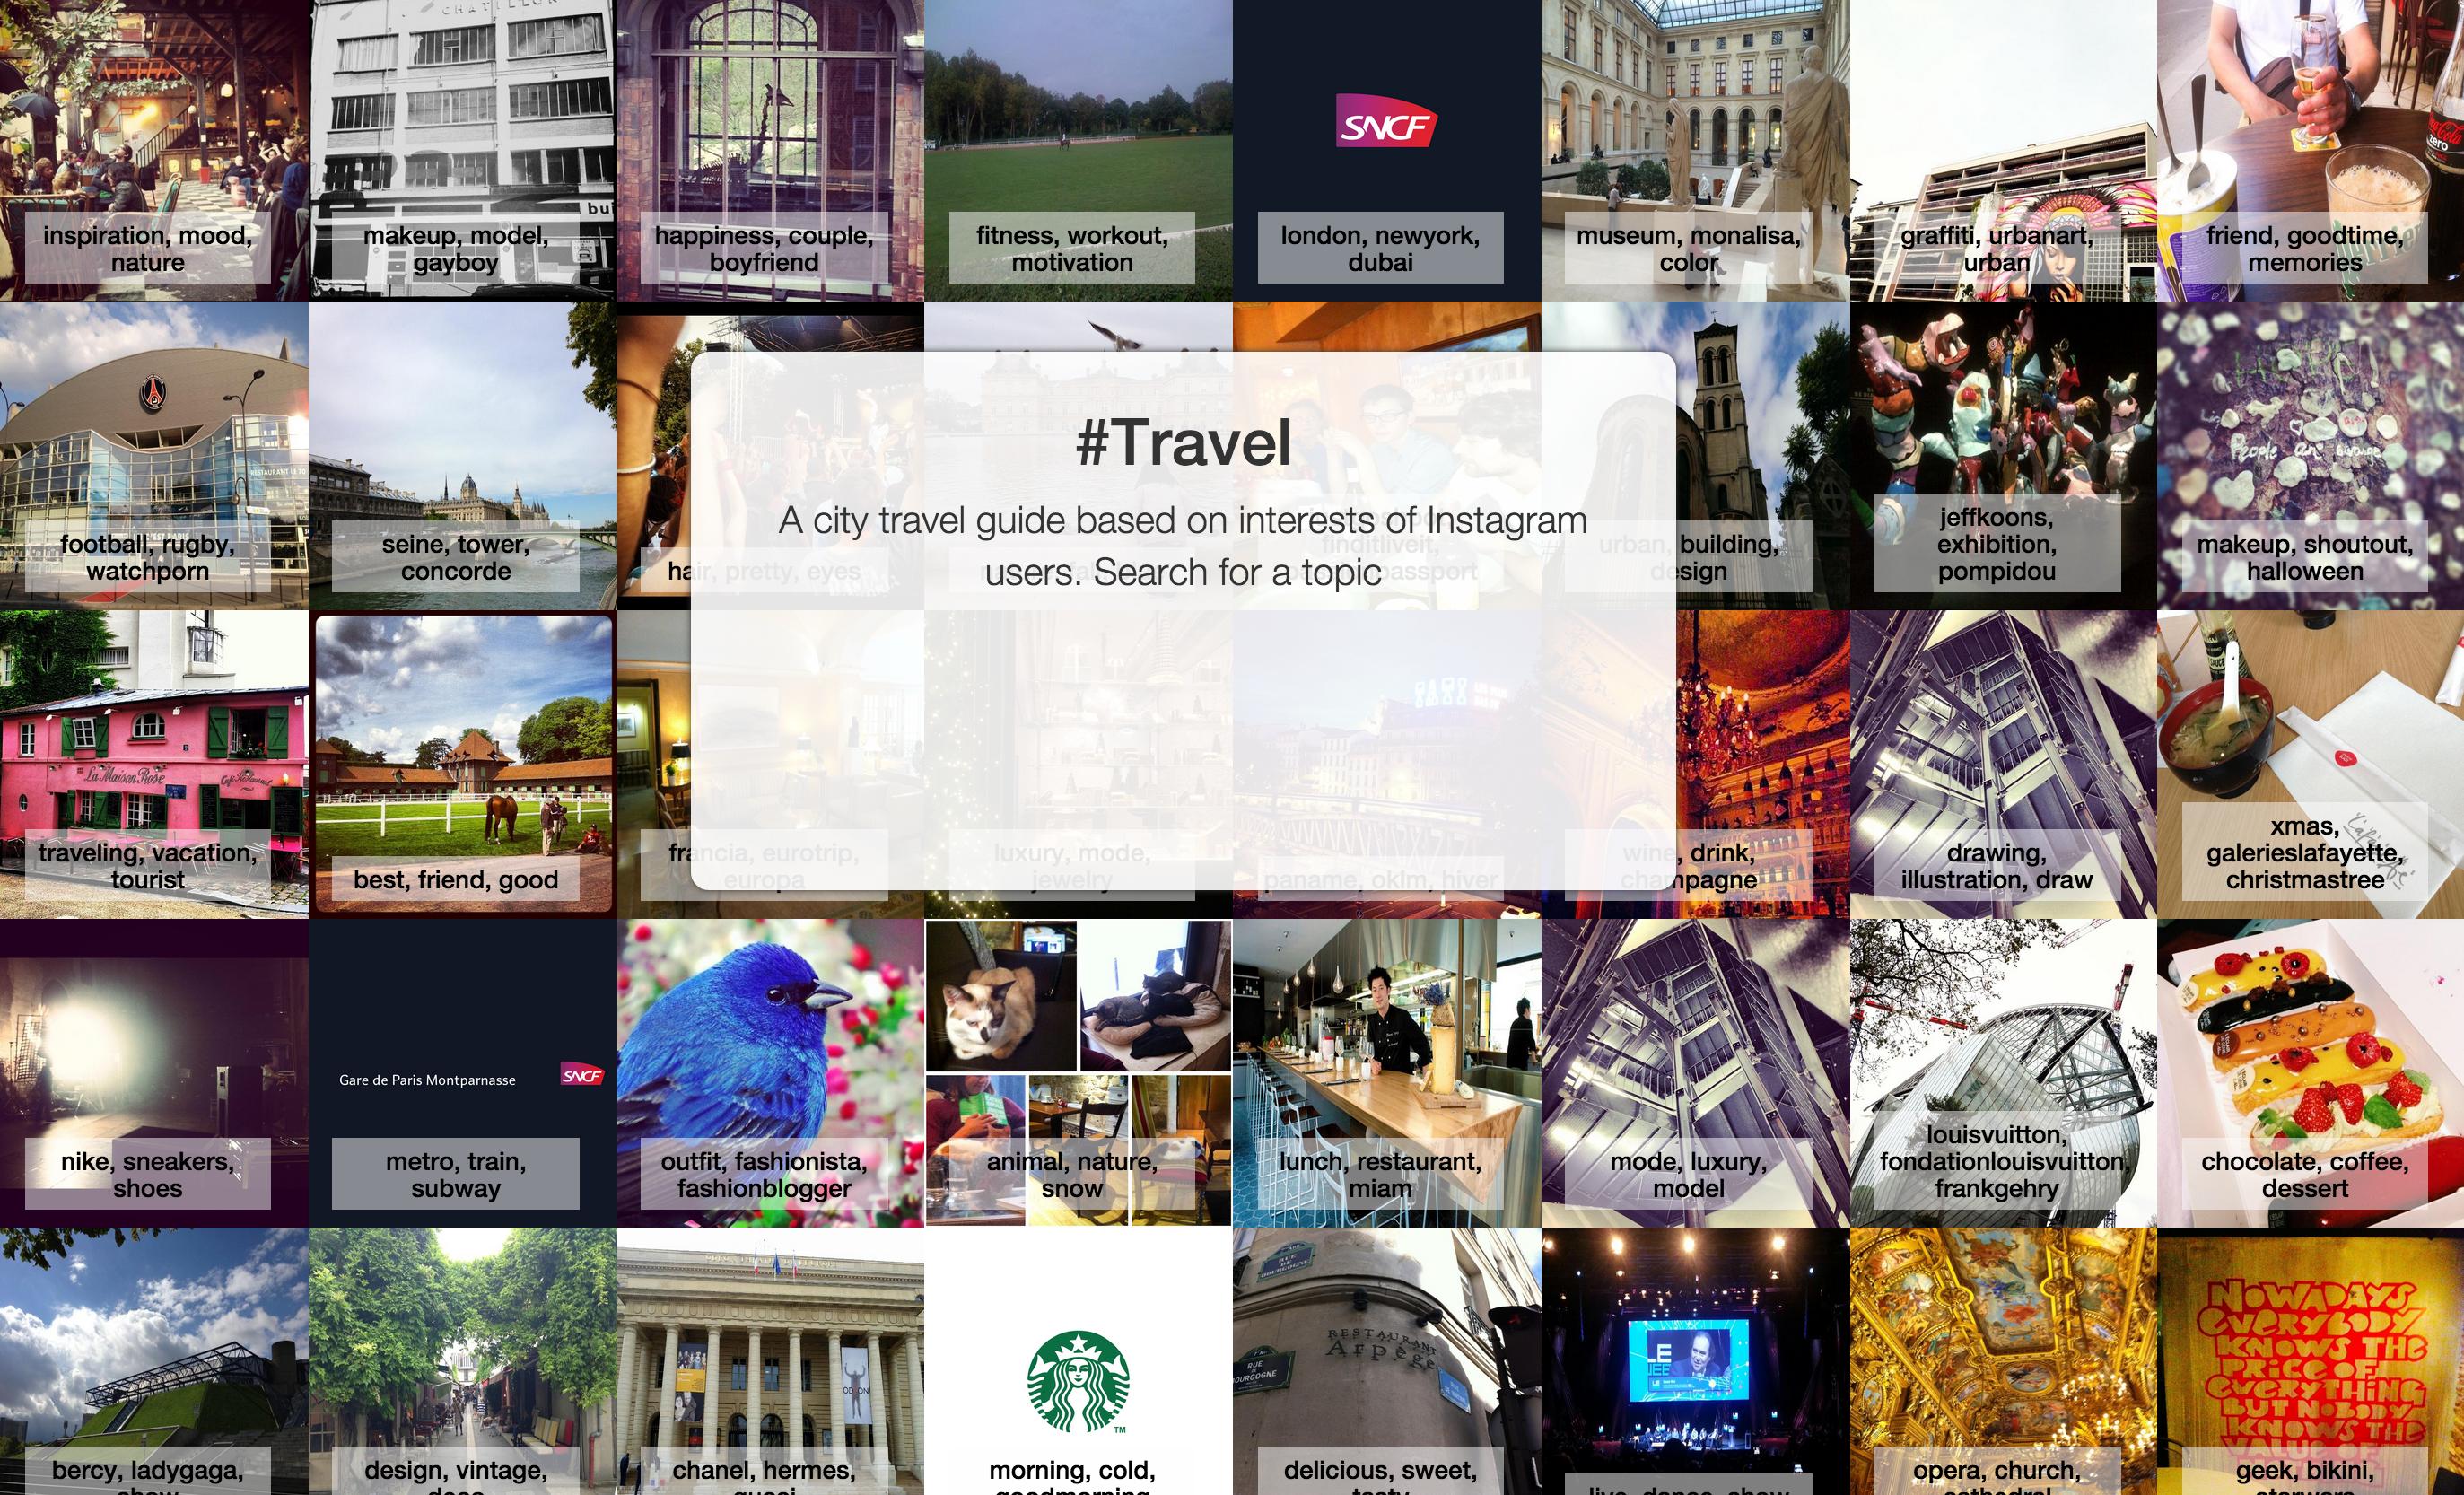
\includegraphics[width=1\textwidth]{images/title}
  \caption{Title page of \#Travel}
  \label{fig:title}
\end{figure}

\begin{figure}[h!]
  \centering
    \includegraphics[width=1\textwidth]{images/map}
  \caption{A set of locations for the topic "Seine, tower, concorde"}
  \label{fig:map}
\end{figure}

\section{Results}
In table \ref{table:results}, we listed the $40$ different extracted topics. For each topic, we list the set of $5$ locations together with the associated category. The algorithm is indeed capable of extracting topics that could interest travellers. Some topics are seasonal, such as "nature, fall, blue", "xmas, galerieslafayette, christmastree" or "animal, nature, snow". Some topics are typical traveling themes: "wine, drink, champagne", "design, vintage, deco", "luxury, mode, jewelry" or "chanel, hermes, gucci". There are some city specific topics, such as "museum, monalisa, color" or "football, rugby, watchporn", "seine, tower, concorde" as well as "jeffkoons, exhibition, pompidou". There is also a lot of noise due to the target group posting on instagram: "best, friend, good", "hair, pretty, eyes", "justgoshoot, finditliveit, passionpassport". On the location side, it is quite hard to judge, because we do not know the places and their characteristics. Some topics have a very appropriate fit, such as "chocolate, coffee, dessert": The recommendation includes a Café, a Dessert Shop, a Chocolate Shop, an Art Gallery as well as A Bio Grocery Store. The topic "design, vintage, deco" includes in its recommendations a flea market, a café place well known for the interior design and a history site. The brand topic includes Chanel and Louboutin whereas the christmas topic proposes a Christmas market. Generally speaking, the recommendations are interesting and for some topics quite appropriate. Engineering additional features, such as distance and popularity could improve the results furthermore.

\begin{longtable}{|p{2in}|p{3in}|}
  \hline \multicolumn{1}{|c|}{\textbf{Topic}} & \multicolumn{1}{c|}{\textbf{Locations (category)}} \\ \hline 
  \endhead

  \caption{Results of the workflow} \label{table:results} \\
  \endfoot
  inspiration, mood, nature & Le Timgad (Moroccan Restaurant), Hyotan (Japanese Restaurant), Paris London Café (French Restaurant), Le Comptoir Général (Bar), Events Management School (Trade School) \\ \hline 
  makeup, model, gayboy & Pin-up Studio (Building), Musée du Louvre (Art Museum), Hapimag Resort Paris (Hotel), Paris   Beaubourg (Café), Studio 217 - Euro Media (Recording Studio) \\ \hline 
  happiness, couple, boyfriend & Pavillon Dauphine (Event Space), Place de Varsovie (Plaza), La Maison de l'Escargot (Gourmet   Shop), Musée du Louvre (Art Museum), Appart'Valley Les Jardins du Roy Residence Paris (Hotel) \\ \hline 
  fitness, workout, motivation & Polo de Paris (Athletics and Sports), Palais des Sports Marcel-Cerdan (Basketball Stadium),  Shangri-La Hotel Paris (Hotel), La Seine (River), Ateliers d'Artistes (Art Gallery) \\ \hline 
  london, newyork, dubai & Comme des coiffeurs (Salon / Barbershop), Kitsuné (Boutique), Guimi-house (Tea Room), Restaurant de  l'Institut du Monde Arabe. (Middle Eastern Restaurant), Gare SNCF de Paris Lyon (Train Station) \\ \hline 
  museum, monalisa, color & Apple Store Carrousel du Louvre (Electronics Store), cour Puget (History Museum), Mona Lisa, L. da  Vinca (Art Museum), Musée National Gustave-Moreau (Museum), Hard Rock Cafe Paris (American Restaurant) \\ \hline 
  graffiti, urbanart, urban & Espace Fondation EDF (Art Gallery), Hôtel Lenox Saint Germain (Hotel), Point Éphémère (Bar),  Parc de Belleville (Park), Rue de Ménilmontant (Street) \\ \hline 
  friend, goodtime, memories & Polo de Paris (Athletics and Sports), La Machine du Moulin Rouge (Music Venue), Musée du Louvre (  Art Museum), La Ferme (Coffee Shop), Les Docks de Paris (Convention Center) \\ \hline 
  football, rugby, watchporn & Parc des Princes (Soccer Stadium), Parc des Princes (Soccer Stadium), Tignes val claret (  Mountain), Stade de France (Stadium), Le Citizen Hotel Du Canal Paris (Hotel) \\ \hline 
  seine, tower, concorde & Arrêt Radio France - Pont de Grenelle [72] (Bus Stop), Grande Roue de Paris (Theme Park Ride /   Attraction), Pont d'Arcole (Bridge), Square de la Tour Saint-Jacques (Park), Place de la République (Plaza) \\ \hline 
  hair, pretty, eyes & Christian Louboutin (Shoe Store), Gare SNCF de Paris Saint-Lazare (Train Station), Hôtel California  Saint-Germain (Hotel), Jamel Comedy Club (Comedy Club), Glazart (Music Venue) \\ \hline 
  nature, fall, blue & The Timhotel Opéra Blanche Fontaine (Hotel), Jardin du Luxembourg (Garden), Assemblée des Départements   de France - ADF (Building), Jardin des Plantes (Botanical Garden), Parc des Buttes-Chaumont (Park) \\ \hline 
  justgoshoot, finditliveit, passionpassport & La Seine (River), Chez Sofia (Middle Eastern Restaurant), Pont Neuf (Bridge),  Église Saint-Eustache (Church), Musée des Arts Forains (Museum) \\ \hline 
  urban, building, design & Église Saint-Pierre de Montmartre (Church), Rue Lafayette (Street), Mercure Paris Boulevard   Magenta (Hotel), Promenade Plantée (Park), bus 89 et arrêt bibliothèque François Mitterrand. (Bus Line) \\ \hline 
  jeffkoons, exhibition, pompidou & Le YOYO (Nightclub), Palais de Tokyo (Cultural Center), Exposition Niki de Saint Phalle ( Other Event), Grand Palais (Historic Site), Jeu de Paume (Art Museum) \\ \hline 
  makeup, shoutout, halloween & Tiffany and Co (Jewelry Store), Les sourires de Dante (Bistro), Apostrophe Hotel (Hotel), The   Thistle (Pub), Tombe de Jim Morrison (Cemetery) \\ \hline 
  traveling, vacation, tourist & Le Timgad (Moroccan Restaurant), La Maison Rose (French Restaurant), Devialet (Electronics   Store), Galerie du Chevalier (Gift Shop), RER Saint-Michel – Notre-Dame [B, C] (Train Station) \\ \hline 
  best, friend, good & Haras de Jardy (Racetrack), Polo de Paris (Athletics and Sports), Parisjob (Building), Hyotan (Japanese  Restaurant), Kyriad Paris IX Montmartre Hotel (Hotel) \\ \hline 
  francia, eurotrip, europa & Château de Versailles (Castle), Palais des Congrès de Versailles (Convention Center), Hôtel   Bedford (Hotel), Aesop (Cosmetics Shop), Les Plumes Hotel (Hotel) \\ \hline 
  luxury, mode, jewelry & Parc des expositions de la Porte de Versailles (Convention Center), CHANEL Boutique (Boutique),   DAVIDOR (Jewelry Store), InterContinental Paris Le Grand Hôtel (Hotel), Café Bords de Seine (Café) \\ \hline 
  paname, oklm, hiver & Gare SNCF de Paris Montparnasse (Train Station), Moulin Rouge Restaurant (French Restaurant), Bar du  Louxor (Café), Anika (Indian Restaurant), Plombier paris 19 (Building) \\ \hline 
  wine, drink, champagne & Place Blanche (Plaza), Le Carmen (Nightclub), Moulin Rouge Restaurant (French Restaurant), Le  Ballroom (Cocktail Bar), Le Comédia (Comedy Club) \\ \hline 
  drawing, illustration, draw & Métro Boucicaut [8] (Subway), École Nationale Supérieure des Beaux-Arts (ENSBA) (College Arts   Building), Théâtre de Paris (Theater), École de la Chambre Syndicale de la Couture (University), Little Red Door (Cocktail  Bar) \\ \hline 
  xmas, galerieslafayette, christmastree & Chalet Sony (Christmas Market), Paroisse Saint-Louis d'Antin (Church), Brasserie du  Printemps (French Restaurant), Paris-Tokyo (Sushi Restaurant), Rue Bichat (Street) \\ \hline 
  nike, sneakers, shoes & Tignes val claret (Mountain), Palais des Sports Marcel-Cerdan (Basketball Stadium), Citadium  Caumartin (Department Store), Paroisse Saint-Louis d'Antin (Church), Maison de l'Architecture d'Ile-de-France (Event Space)  \\ \hline 
  metro, train, subway & Hotel Mercure Paris Arc de Triomphe Etoile (Hotel), Gare SNCF de Paris Montparnasse (Train Station),   Au Petit Montmartre (Café), Métro Marcadet Poissonniers [4, 12] (Subway), Starbucks (Coffee Shop) \\ \hline 
  outfit, fashionista, fashionblogger & UMA (Japanese Restaurant), Mercure Paris Montmartre (Hotel), Théâtre de Paris ( Theater), paris chez vous (Bed and Breakfast), Musée des Arts et Métiers (Museum) \\ \hline 
  animal, nature, snow & Mairie de Neuilly-sur-Seine (City Hall), Rue du Bac (Street), Cimetière du Montparnasse (Cemetery),  Gymnase Michel Le Comte (General Entertainment), Café de l'Industrie (Bistro) \\ \hline 
  lunch, restaurant, miam & Les Cocottes (French Restaurant), Kunitoraya 1 rue Villedo (Ramen / Noodle House), Merci (  Department Store), Pierre Sang in Oberkampf (Restaurant), Starvin' Joe (Burger Joint) \\ \hline 
  mode, luxury, model & Citadium Caumartin (Department Store), Montmartre (Neighborhood), Lagostore Paris Sentier (Furniture /  Home Store), École de la Chambre Syndicale de la Couture (University), UNIQLO Le Marais (Clothing Store) \\ \hline 
  louisvuitton, fondationlouisvuitton, frankgehry & Fondation Louis Vuitton (Art Museum), Jardin d'Acclimatation (Theme Park),  Fondation Louis Vuitton (Art Museum), Fondation Louis Vuitton (Art Museum), Le Theatre du Jardin D'acclimatation (General  Entertainment) \\ \hline 
  chocolate, coffee, dessert & Café Kitsuné (Café), L'Éclair de Génie (Dessert Shop), Chocolaterie Jacques Genin (Chocolate   Shop), La Cartonnerie (Art Gallery), Belleville En Bio (Grocery Store) \\ \hline 
  bercy, ladygaga, show & Palais des Sports (Comedy Club), Île de la Cité (Island), Cirque d'Hiver Bouglione (Circus), Le   Bataclan (Concert Hall), Palais omnisports de Paris-Bercy (Music Venue) \\ \hline 
  design, vintage, deco & Ma Cocotte (French Restaurant), Le Paul Bert (Café), Marché aux puces de Saint-Ouen (Flea Market),  Rue Pastourelle (Street), Carreau du Temple (Historic Site) \\ \hline 
  chanel, hermes, gucci & Pavillon Dauphine (Event Space), Christian Louboutin (Shoe Store), CHANEL Boutique (Boutique), Arrêt  Théâtre de l'Odéon [58] (Bus Stop), Odéon – Théâtre de l'Europe (Theater) \\ \hline 
  morning, cold, goodmorning & Starbucks (Coffee Shop), Select Rive Gauche (Hotel), Paris-Sorbonne University (11 SHS) (  College Academic Building), Bibliotheque Universitaire Censier (College Library), Université Paris VIII - Vincennes Saint-  Denis (University) \\ \hline 
  delicious, sweet, tasty & L'Arpège (Vegetarian / Vegan Restaurant), Paris en Scène (Boat or Ferry), Niji Sushis (Asian  Restaurant), Paris HQ (Miscellaneous Shop), L'Éclair de Génie (Dessert Shop) \\ \hline 
  live, dance, show & Théâtre Mogador (Theater), Alice Pizza Dancourt (Pizza Place), Le Trianon (Concert Hall), LeWeb 2014 (  Conference), Grande Halle de la Villette (Event Space) \\ \hline 
  opera, church, cathedral & Piscine molitor (Restaurant), Opéra Garnier (Opera House), Sainte-Chapelle (Church), Musée   national du Moyen-Âge (History Museum), La Conciergerie (Historic Site) \\ \hline 
  geek, bikini, starwars & Toys"R"Us (Toy / Game Store), Place de la Porte de Saint-Cloud (Plaza), Marché Aux Fleurs (Flower  Shop), Quartier Drouot (Neighborhood), Le Quinze (Bar) \\ \hline 

  \hline
\end{longtable}

\section{Conclusion and future work}

From a student point of view, this project was highly interesting. During the project, I walked through the following points:
\begin{enumerate}
  \item Think about the necessary data and possible data sources, retrieve enough data
  \item Characterize the data using exploratory data science
  \item Apply suitable techniques (DBSCAN, BTM) in order to make the data usable
  \item Mash up data with other data sources
  \item Engineer a work flow that generates a final result (sets)
  \item Build a web application that allows users to interact with the final result 
\end{enumerate}
Nevertheless, there is still a lot of work to be done in order to make the workflow more efficient and more suitable to the needs of users. For future work, the batch processing could be ported to real-time, using incremental versions of both DBSCAN and BTM algorithms. As a result, real-time events happening in a city could be detected and suitable lists of locations recommended. A qualitative and quantitative evaluation process of the generated sets should be put in place, such that further improvements of the algorithm can be measured quantitatively. Furthermore, we suggest improvements in the set generation algorithm, taking into account additional features, such as distance and popularity.

\newpage
\nocite{*} 


\bibliographystyle{unsrtnat} 

\bibliography{references}
\clearpage
\begin{appendix}
\addcontentsline{toc}{chapter}{APPENDICES}
\chapter{LDA Appendix}

\begin{enumerate}
  \item lifestyle,coffee,chocolate
  \item hair,pretty,nice,funny,eyes,time
  \item enjoy,today,happiness
  \item luxury,oklm,paname
  \item miss
  \item color,moment,fashionblogger
  \item holidays,landscape
  \item december,gift,lunch
  \item with
  \item fall,blonde
  \item shoes
  \item morning,school
  \item gold,bijoux,jewelry
  \item nike,london
  \item model,halloween
  \item fitness
  \item motivation
  \item handmade
  \item miam,tour
  \item champselysees
  \item sweet
  \item work
  \item colors,green
  \item home,drawing
  \item sunset,shooting,wine
  \item cold,baby
  \item restaurant,good
  \item design,inspiration,outfit
  \item francia
  \item perfect
  \item designer,boulogne,teatime
  \item museum
  \item vintage,saturday
  \item mode,xmas,metro
  \item chill,cake
  \item vacation
  \item live,chanel
  \item friend,best
  \item luxe,lips,madeinfrance
  \item makeup,nature,blue,pink
\end{enumerate}
\end{appendix}

\end{document}